\section{Controlli semantici}

I controlli semantici effettuati sono quelli elencati sotto:
\begin{itemize}
   \item non è possibile re-dichiarare una classe
   \item non è possibile re-dichiarare una metodo (con stessa segnatura) in una
   classe
   \item i nomi degli attributi di un metodo non si possono ripetere nella stessa dichiarazione
   \item non è possibile re-dichiarare una relazione in una classe (ugual tipo,
   sorgente, destinazione)
   \item non è possibile re-dichiarare un attributo in una classe (ugual tipo e
   nome)
   \item non è possibile inserire la stessa classe in un diagramma 
\end{itemize}


I controlli vengono effettuati con due modalità: quando i dati devono essere
verificati localmente vengono passati sull'albero, mentre se sono dati che vanno
raccolti per tutto l'albero e poi controllati alla radice vengono gestiti per
mezzo di variabili globali.

Esempi di variabili globali sono la lista delle classi dichiarate, delle
relazioni dichiarate, delle classi contenute nel diagramma; mentre vengono passati
sull'albero la
definizione dei Gruppi, delle Classi, degli Attributi, dei Metodi.
Per effettuare i controlli sono stati definite delle funzioni semantiche
all'interno del file ``.cc''.

\begin{figure}[htp]
\begin{center}
  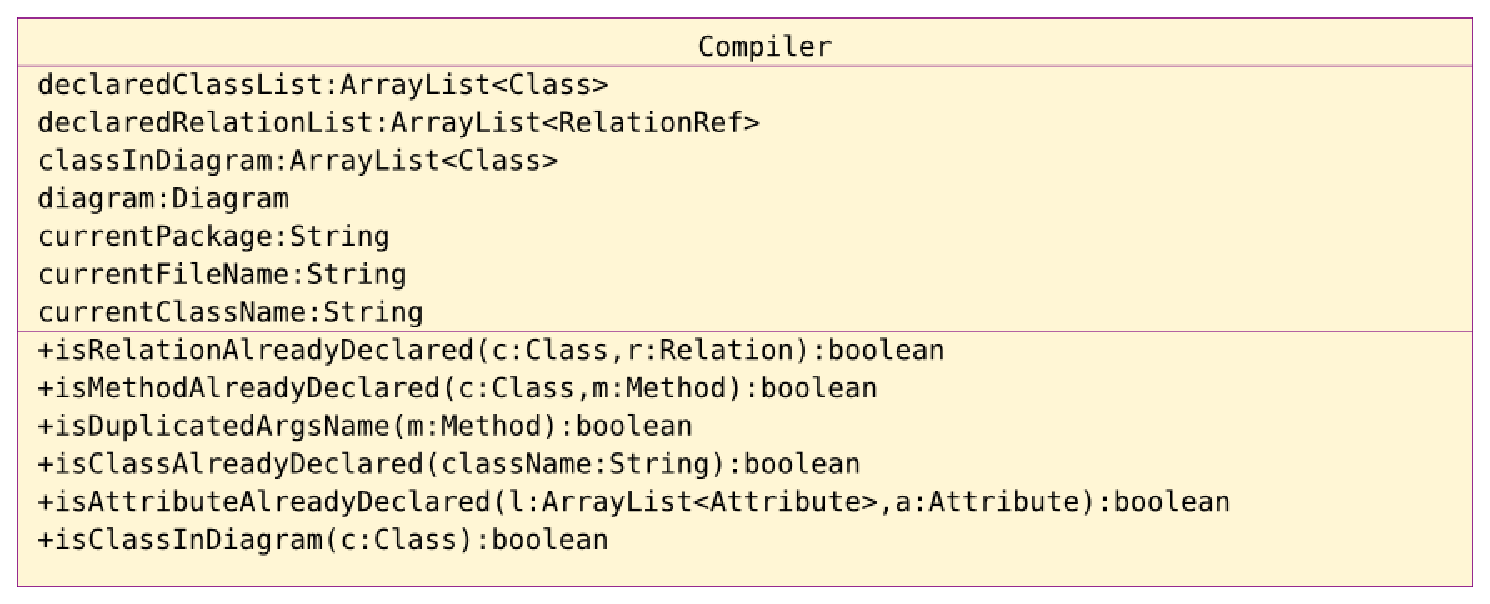
\includegraphics[width=0.9\textwidth]{img/uml_compilatore}
  \caption[labelInTOC]{Struttura del codice per l'esecuzione dei controlli semantici.}
\end{center}
\end{figure}

Nel diagramma uml soprastante\footnote{Il digramma è stato creato con cUml2Svg} sono
indicate le strutture dati e le funzioni di supporto per i controlli semantici.
In questa implementazione nessun controllo semantico blocca la compilazione,
viene visualizzato il messaggio di errore ma il diagramma viene comunque
generato; è stato scelto questo comportamento per fare in modo di visualizzare
tutti gli errori oltre a permettere ad un utente esperto (che conosce il
funzionamento della generazione del diagramma) di utilizzare il sistema in
situazioni particolari come per esempio l'import di modelli multipli e sovrapposti.
